\section*{Βήμα 0}
Εκτελούμε το κομμάτι κώδικα που μας δίνεται στην εκφώνηση. Το αποτέλεσμα (υποφάκελοι) φαίνεται παρακάτω:

\begin{figure}[H]
	\centering
	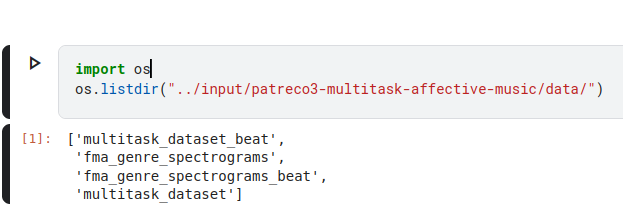
\includegraphics[width=0.6\linewidth]{images/prep_step0.png}
\end{figure}

\noindent Ενεργοποιώντας και απενεργοποιώντας την GPU από το μενού στα δεξιά του Notebook, βλέπουμε ότι έχουμε 30 ώρες εβδομαδιαίως για να μπορούμε να την χρησιμοποιούμε. Οι επιλογές των accelerator που μας δίνονται είναι:

\begin{itemize}
	\item GPU T4x2
	\item GPU P100
	\item TPU v5e-8
\end{itemize}

\section*{Βήμα 1}
\subsection*{Ερώτημα α}
Στο ερώτημα αυτό μας ζητείται να διαβάσουμε 2 τυχαίες γραμμές με διαφορετικές επισημειώσεις. \\

\noindent Διαβάζουμε το αρχείο αυτό σε ένα Pandas Dataframe και στη συνέχεια το χρησιμοποιούμε για να πάρουμε ένα δείγμα από κάθε κατηγορία - τυχαία. Έτσι και μπορούμε να επιλέξουμε 2 διαφορετικές γραμμές με διαφορετικό label και μαθαίνουμε ποιες είναι οι πιθανές επισημειώσεις των δεδομένων μας. Ο κώδικας και το αποτέλεσμά του φαίνονται στην επόμενη σελίδα. \\

\noindent Επιλέγουμε προς ανάγνωση το Hip-Hop και το Punk κομμάτι. 

\begin{figure}[H]
	\centering
	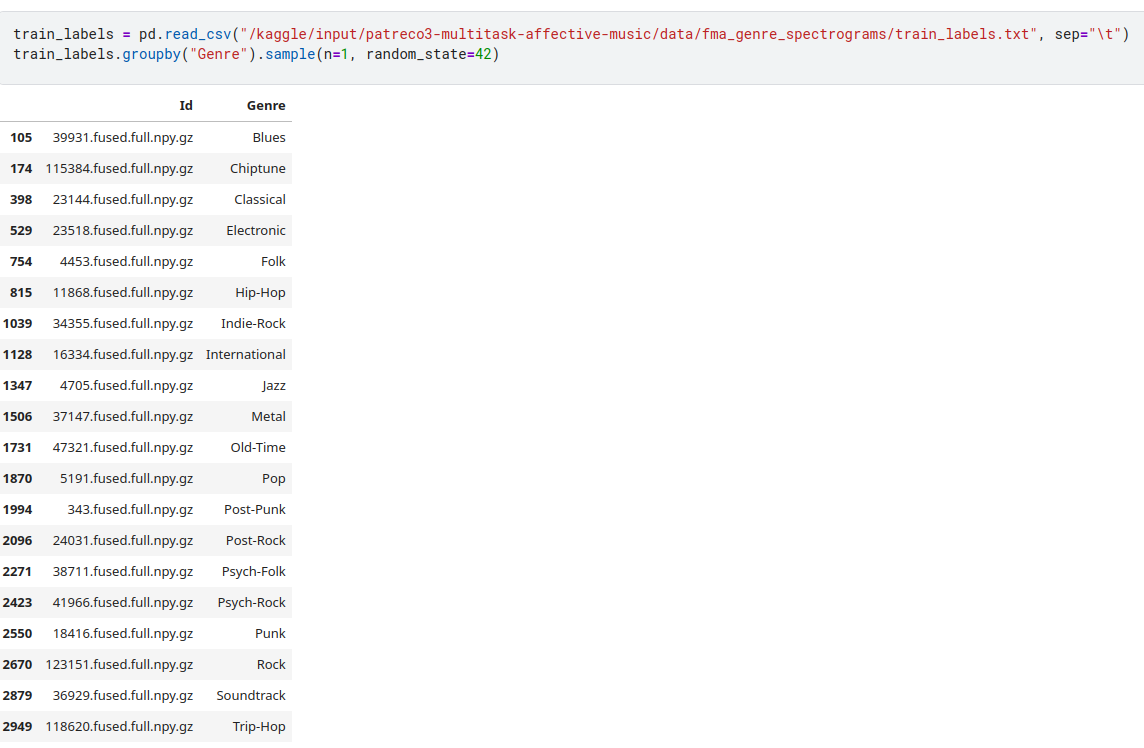
\includegraphics[width=0.75\linewidth]{images/prep_step1a_readlabels.png}
\end{figure}

\subsection*{Ερώτημα β}
Σύμφωνα με το κώδικα που μας δόθηκε στην πρώτη βιβλιογραφική αναφορά, διαβάζουμε τα φασματογραφήματα των 2 κομματιών που επιλέξαμε και τυπώνουμε τις διαστάσεις τους ώστε να ελέγχξουμε κατά πόσο η ανάγνωση ήταν επιτυχημένη.

\begin{figure}[H]
	\centering
	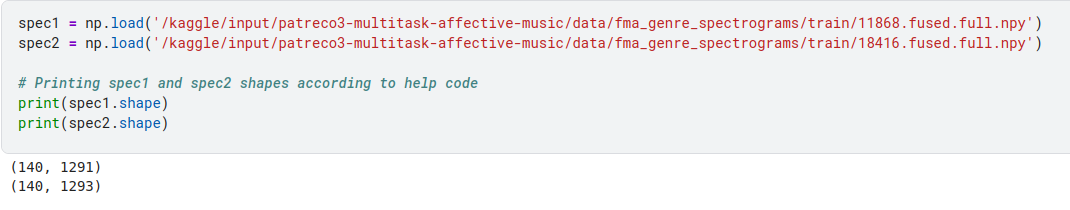
\includegraphics[width=0.75\linewidth]{images/prep_step1b_readspec.png}
\end{figure}

\noindent Από το βοηθητικό αρχείο μαθαίνουμε ότι τα δείγματα είναι μία συνένωση mel spectrogram και chromagram. Συγκεκριμένα, οι πρώτες 128 (από τις 140) "συχνότητες" αφορούν τα 128 mel frequency bands (συχνότητες που αντιλαμβάνεται ο άνθρωπος) και οι τελευταίες 12 οι 12 pitch κλάσεις του chromagram.

\begin{figure}[H]
	\centering
	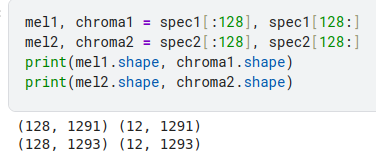
\includegraphics[width=0.4\linewidth]{images/prep_step1b_melchroma.png}
\end{figure}

\subsection*{Ερώτημα γ}

Συνεχίζοντας να ακολουθούμε το κώδικα που μας δίνεται, απεικονίζουμε το spectrogram με τη συνάρτηση που μας ζητείται και τα απεικονίζουμε στην επόμενη σελίδα. \\

\noindent Ο κατακόρυφος άξονας του spectrogram αντιστοιχεί στις συχνότητες του σήματος ενώ ο οριζόντιος στο χρόνο. Πρακτικά, κάνουμε έναν συχνοτικό μετασχηματισμό (dft, mel filterbank,...) κάθε χρονική στιγμή και με την ένταση του χρώματος δείχνουμε το μέγεθος του εκάστοτε συχνοτικού περιεχομένου.

\begin{figure}[H]
	\centering
	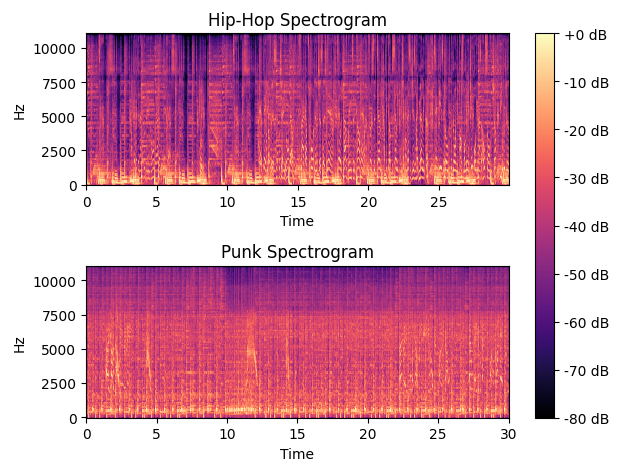
\includegraphics[width=0.7\linewidth]{images/prep_step1c_spectrograms.png}
\end{figure}

\noindent Το πρώτο σχόλιο που αξίζει να κάνουμε για να συγκρίνουμε τα 2 διαγράμματα, αφορά στην κατανομή της ισχύος των σημάτων στις συχνότητές τους. Στη hip-hop μουσική, όπως γνωρίζουμε, κυριαρχούν τα μπάσα και οι χαμηλές συχνότητες, ενώ στη μουσική punk ο ρυθμός και η ένταση είναι πιο ακατάστατα, οπότε αναμένουμε να υπάρχει μια κάπως πιο ομοιόμορφη κατανομή της ισχύος σε όλες τις συχνότητες. 

\noindent Πράγματι, οι προσδοκίες μας επιβεβαιώνονται από τα διαγράμματα, αφού στο spectrogram του hip-hop τα έντοντα κίτρινα (μπορούμε να το επιβεβαιώσουμε στο colorbar), δηλαδή το μεγαλύτερο ποσό της ισχύος βρίσκεται συγκεντρωμένο στις συχνότητες κάτων των 2500Hz. Από την άλλη, στην punk πρακτικά έχουμε κάλυψη των συχνοτήτων μέχρι τα 7500Hz σχεδόν ομοιόμορφα ενώ παρόλο που είναι λιγότερο έντονο, υπάρχει συχνοτικό περιεχόμενο και στις πολύ υψηλές συχνότητες. \\

\noindent Επίσης, η hip-hop μουσική είναι πιο ρυθμική. Για αυτό εξετάζοντας την εξέλιξη του συχνοτικού περιεχομένου κατά τον οριζόντιο άξονα-χρόνο βλέπουμε ότι σχηματίζονται λωρίδες παρουσίας-απουσίας συχνοτικού περιεχομένου. Αυτό δεν συμβαίνει στην punk εξαιτίας του χάους και της απουσίας ξεκάθαρης ρυθμικότητας που την χαρακτηρίζουν. Το συχνοτικό περιεχόμενο είναι κάπως ομοιόμορφο στην χρονική εξέλιξη του σήματος.

\subsection*{Ερώτημα δ}
Το ανθρώπινο αυτί δεν αντιλαμβάνεται γραμμικά και ομοιόμορφα τις διάφορες συχνότητες των σημάτων. Παρουσιάζει κατά βάση μεγαλύτερη ευαισθησία στις χαμηλές συχνότητες ενώ μικρότερη στις υψηλότερες συχνότητες. \\

\noindent Αυτό ώθησε στη δημιουργία μίας αντιληπτικής κλίμακας συχνοτήτων. Δηλαδή, μιας κλίμακας που να είναι γραμμική με τον τρόπο τον οποίο το αυτί μας αντιλαμβάνεται τις συχνότητες. Αυτή είναι η κλίμακα Mel (από τη λέξη melody). \\

\noindent Όπως διαβάζουμε και σε αυτό το \href[]{https://en.wikipedia.org/wiki/Mel_scale}{άρθρο}, η Mel scale είναι αποτέλεσμα μιας σειράς ψυχοακουστικών πειραμάτων που διεξήγαγαν οι S. S. Stevens, J. Volkman και E. Newman το 1937. Στα πειράματα αυτά πρακτικά δινόταν στους συμμετέχοντες ένας ήχος από μία και μόνο συχνότητα, έστω 2000Hz. Στη συνέχεια έπρεπε να τον ρυθμίσουν ώστε το pitch να ακούγεται υποδιπλάσιο ή υπερδιπλάσιο. \\

\noindent Έτσι, επιβεβαιώθηκε η απουσία γραμμικής συσχέτισης συχνότητας και αντίληψής της από τον άνθρωπο, αφού οι αλλαγές για παράδειγμα από τα 100Hz στα 200Hz ακουγόταν πολύ μεγαλύτερες από εκείνες των 5000Hz στα 5100Hz. Επιπλέον, τα δεδομένα που είχαν συλλεχθεί σε μορφή πινάκων οδήγησαν στη σχέση μεταξύ κλίμακας Mel και Hz, με μία από τις πιο πρόσφατες εκδοχές της να είναι:

$$m = 2595\log_{10}\left(1+\frac{f}{700}\right)$$ 

\begin{figure}[H]
	\centering
	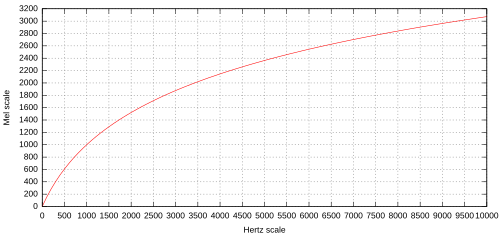
\includegraphics[width=0.7\linewidth]{images/mel.png}
\end{figure}

\noindent Η κλίμακα Mel χρησιμοποιείται σε πληθώρα εφαρμογών επεξεργασίας σήματος ήχου και φωνής. Πρώτα από όλα, μετασχηματίζει τις συχνότητες με τρόπο που δίνεται έμφαση στις χαμηλότερες σε σχέση με τις ψηλότερες μιμούμενο την ανθρώπινη ακοή. Επιπλέον, είναι χρήσιμο γιατί με αυτό τον τρόπο μπορούμε να απομονώσουμε τα πιο σημαντικά κομμάτια ενός ηχητικού σήματος με κριτήριο την ευκρινέστερη αντίληψή τους από τους ακροατές. Έτσι, μπορεί να λειτουργήσει ως μέθοδος μείωσης διαστατικότητας τέτοιων σημάτων. Κατά κάποιο τρόπο αυτός είναι και ο λόγος για τον οποίο η κλίμακα αυτή λειτουργεί ως φίλτρο, αφού καταπιέζει τον υψίσυχνο θόρυβο. Τέλος, μπορεί κανείς να εξάγει τα Mel Cepstral Coefficients που χρησιμοποιούνται σε πολλές εφαρμογής μηχανικής μάθησης ως διανύσματα χαρακτηριστικών.

\section*{Βήμα 2}
\subsection*{Ερώτημα α}

\begin{itemize}
	\item Όπως φαίνεται και στην πρώτη εικόνα του ερωτήματος β, οι διαστάσεις των 2 spectrograms είναι:
	
	\begin{itemize}
		\item (140, 1291)
		\item (140, 1293)
	\end{itemize}
	
	Οπότε ο αριθμός των χρονικών βημάτων για το spectrogram του hip hop τραγουδιού είναι 1291 ενώ για του αντίστοιχου punk είναι 1293.
	
	\item Η εκπαίδευση ενός LSTM πάνω στα φασματογραφήματα δεν είναι εν γένει αποδοτική για τα spectrograms του συνόλου δεδομένων στην μορφή την οποία βρίσκονται.
	
	\item Το μήκος των ακολουθιών των δειγμάτων (1291 και 1293 αντίστοιχα) είναι αρκετά μεγάλο ώστε να δημιουργήσει προβλήματα vanishing gradient στο δίκτυο. Επιπλέον το backpropagation through time δεν θα είναι αποδοτικό ως προς την ταχύτητα σύγκλισης των παραμέτρων. Για αυτό μια καλή ιδέα θα ήταν να σπάμε τις ακολουθίες σε μικρότερα τμήματα στα οποία θα θέλαμε να επικεντρωθούμε. Αυτό όμως ενδέχεται να επηρεάσει το accuracy του μοντέλου μας. Επιπλέον, ο μεγάλος αριθμός κρυφών καταστάσεων που θα ξεδιπλωθούν είναι πολύ απαιτητικός σε υπολογιστικούς πόρους αλλά και σε μνήμη (RAM ή VRAM για GPU). Καταλήγουμε πως η εκπαίδευση ενός LSTM για το συγκεκριμένο task δεν είναι αδύνατη, αλλά θα χρειαστεί περαιτέρω επεξεργασία στα δεδομένα μας και τροποποίηση του αλγορίθμου εκπαίδευσης.
	
\end{itemize}

\subsection*{Ερώτημα β}

Αρχικά, καλούμαστε να επιλέξουμε τυχαία 2 γραμμές με διαφορετικές επισημειώσεις από το dataset των beatsynced spectrograms. Αυτά βρίσκονται στο αρχείο \textit{/input/patreco3-multitask-affective-music/data/fma\_genre\_spectrogram\_beat}.

\begin{figure}[H]
	\centering
	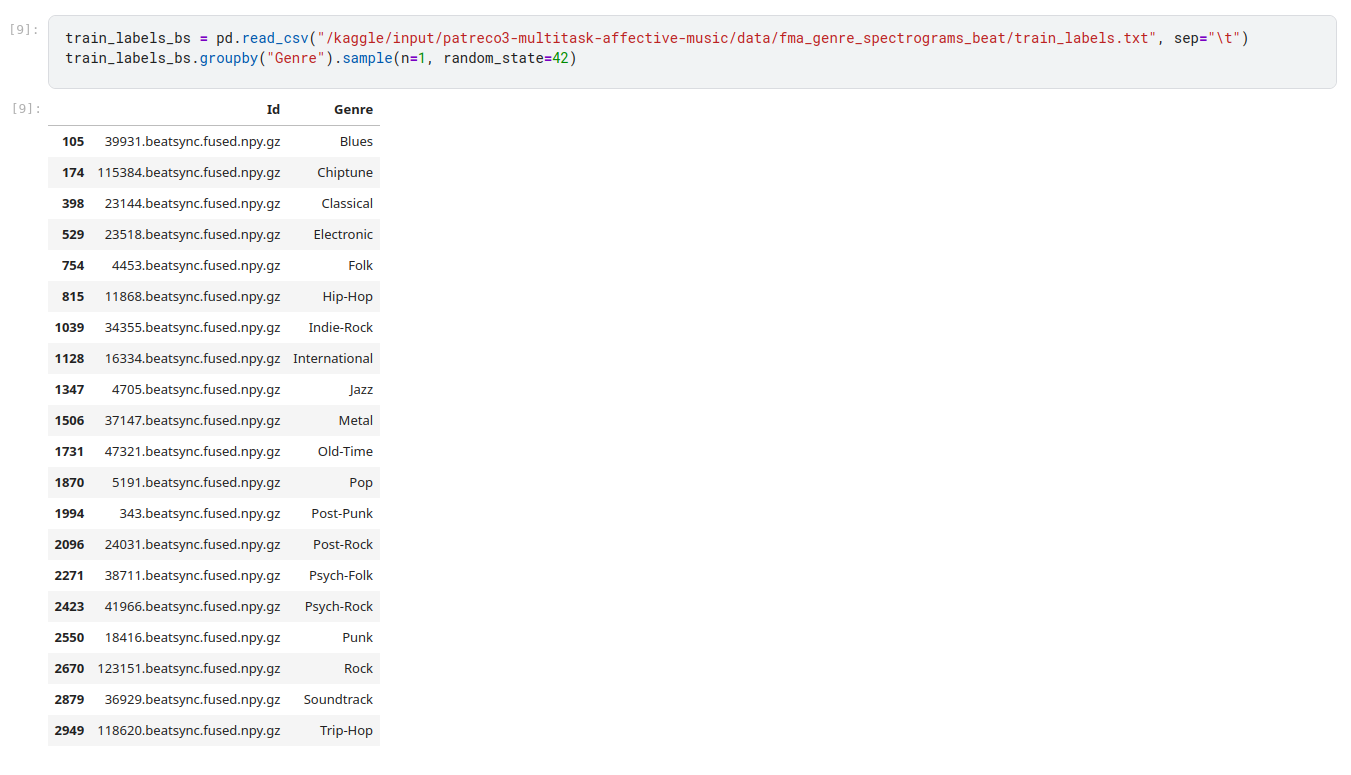
\includegraphics[width=\linewidth]{images/prep_step2b_a.png}
\end{figure}

\noindent Επιλέγουμε πάλι τα τυχαία δείγματα hip-hop και punk προκειμένου να μπορέσουμε να κάνουμε ουσιοδέστερη σύγκριση και σχολιασμό των beat synced με τα αντίστοιχα μη beat synced versions που έχουμε ήδη εξετάσει. \\

\noindent Φορτώνουμε τα αρχεία και διαχωρίζουμε τα spectrograms (πρώτες 128 συχνοτικές συνιστώσες) από τα chromagrams (τελευταίες 12 συνιστώσες) όπως και στο βήμα 1:

\begin{figure}[H]
	\centering
	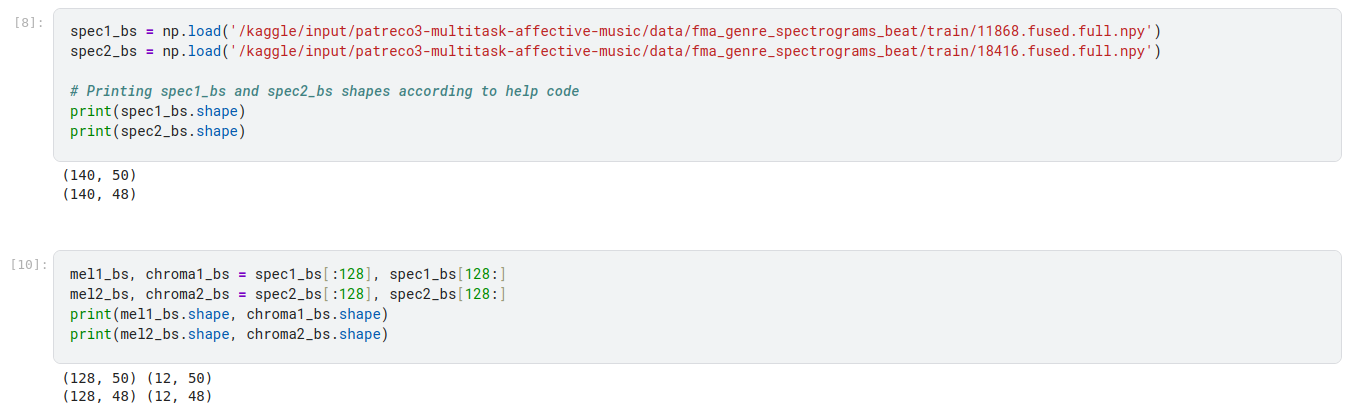
\includegraphics[width=\linewidth]{images/prep_step2b_b.png}
\end{figure}

\noindent Πράγματι, βλέπουμε ότι τα timesteps είναι πολύ λιγότερα (2 τάξεις μεγέθους). Πιο συγκεκριμένα, στο πρώτο βήμα της άσκησης είδαμε πως τα τυχαία μας δείγματα αποτελούνταν από 1291 και 1293 timesteps αντίστοιχα. Τώρα, οι αριθμοί αυτοί είναι 50 και 48 αντίστοιχα. \\

\noindent Αξίζει να σχολιάσουμε πως πλέον τα προβλήματα που αναφέραμε για την εκπαίδευση ενός LSTM πάνω στα spectrograms έχουν λυθεί. Αρχικά θα χρειαστούν πολύ λιγότερες κρυφές καταστάσεις στα μοντέλα και επομένως η κατανάλωση μνήμης θα είναι αισθητά μικρότερη. Το ίδιο ισχύει και για τους υπολογισμούς που απαιτούνται. Επιπλέον, η εκπαίδευση είναι αποδοτικότερη, αφού τα προβλήματα του vanishing gradient και της απώλειας πληροφορίας εξαιτίας μεγάλου context είναι πολύ λιγότερο έντονα σε σχέση με πριν (ή και εντελώς απόντα). \\

\noindent Απεικονίζουμε τα spectrograms με τον ίδιο τρόπο με εκείνο του προηγούμενου βήματος και έχουμε:

\begin{figure}[H]
	\centering
	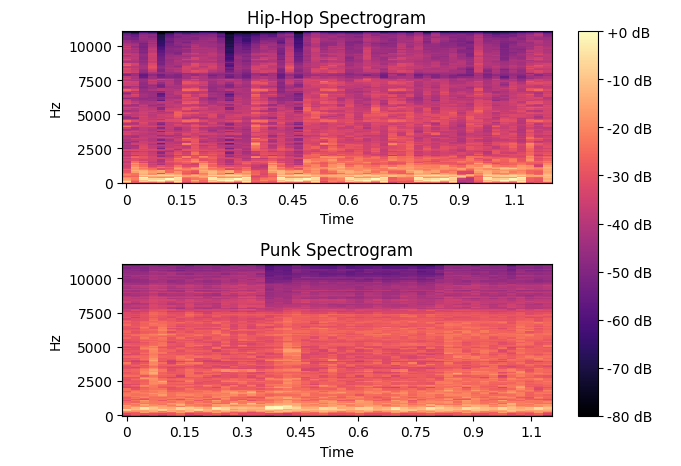
\includegraphics[width=0.7\linewidth]{images/prep_step2b_c.png}
\end{figure}

\noindent Αυτό που παρατηρούμε είναι πως τα διαγράμματα είναι λιγότερο ευκρινή σε σχέση με τα πρώτα. Αυτό είναι αναμενόμενο αφού πληροφορία από διαφορετικά χρονικά timesteps έχει συμπικνωθεί στα σημεία εκείνα που χτυπά το beat της μουσικής με τη χρήση ενός "στατιστικού αντιπροσώπου" τους, του median. Παρόλα αυτά, τα ποιοτικά χαρακτηριστικά των διαγραμμάτων παραμένουν αναλλοίωτα και τα συμπεράσματα που βγάζουμε από αυτά παραμένουν όμοια με πριν. Αυτό σημαίνει ότι αυτή η προσπάθεια μας για αποδοτικό και ουσιαστικό dimensionality reduction είναι μάλλον επιτυχημένη, αφού οι διαστάσεις (timesteps) των χαρακτηριστικών μειώθηκαν αισθητά, αλλά η σημαντική πληροφορία διατηρήθηκε.


\subsection*{Βήμα 3}
Πρακτικά τα chromagrams έχουν ήδη εξαχθεί. Πρόκειται για τις τελευταίες 12 εκ των 140 συνιστωσών των fused αρχείων. Η ανάγνωση και ο διαχωρισμός τους από τα spectrograms φαίνονται αντίστοιχα στο ερώτημα 1β. Η τυχαία επιλογή έγινε ταυτόχρονα με την τυχαία επιλογή των spectrograms στα αντίστοιχα ερωτήματα. \\

\noindent Όσον αφορά τις διαστάσεις των chromagrams έχουμε ότι:

\begin{itemize}
	\item Chromagram Hip-Hop: (12, 1291)
	\item Chromagram Punk: (12, 1293)
	\item Chromagram Beat Synced Hip-Hop: (12, 50)
	\item Chromagram Beat Synced Punk: (12, 48)
\end{itemize}

\noindent Τα chromograms πρακτικά συμπιέζουν την συχνοτική πληροφορία του κομματιού αγνοώντας τις διαφορετικές οκτάβες. Ουσιαστικά, είναι ενδεικτικά της ενέργειας σε κάθε νότα κάθε χρονική στιγμή. \\

\noindent Απεικονίζουμε τα chromagrams σύμφωνα με τον βοηθητικό κώδικα και παίρνουμε:

\begin{figure}[H]
	\centering
	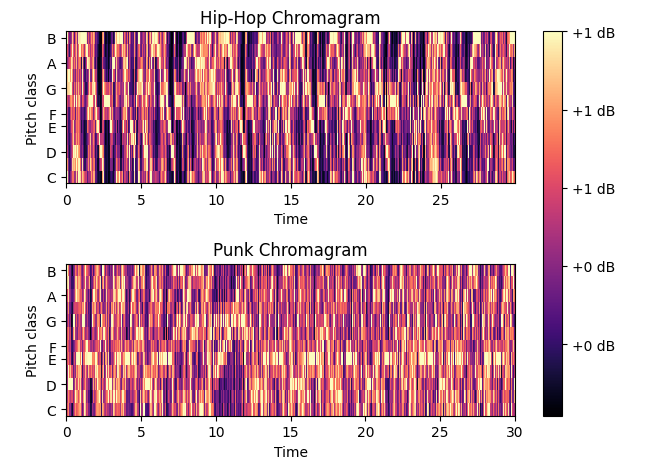
\includegraphics[width=0.7\linewidth]{images/prep_ste3_chromagrams.png}
\end{figure}

\noindent Όπως είναι αναμενόμενο και σε αντιστοιχία με τα σχόλιά μας για τα spectrograms, βλέπουμε ότι το χρωμογράφημα της punk μουσικής είναι πολύ πιο πυκνό και θορυβώδες από το αντίστοιχο της hip hop. Αυτό συμβαίνει διότι στην punk πολλές νότες παίζονται ταυτόχρονα και σε παρόμοια ένταση, σε αντίθεση με τη hip-hop που είναι πιο ρυθμική με σαφείς αλλαγές της μελωδίας και του μπάσου. Επιπλέον, στην περίπτωση της hip-hop μπορεί κανείς να διακρίνει ένα μοτίβο στο plot, ενδεικτικό της επαναληψιμότητας των συνδυασμών από νότες που παίζονται. Κάτι τέτοιο δεν ισχύει για την punk, αφού είναι πιο χαοτική. Τέλος, οι εναλλαγές στην ένταση κάθε νότας είναι πολύ πιο έντονες και απότομες κατά τη διάρκεια του κομματιού στην punk μουσική. \\

\noindent Ακολουθεί το χρωμογράφημα της beat synced εκδοχής των κομματιών:

\begin{figure}[H]
	\centering
	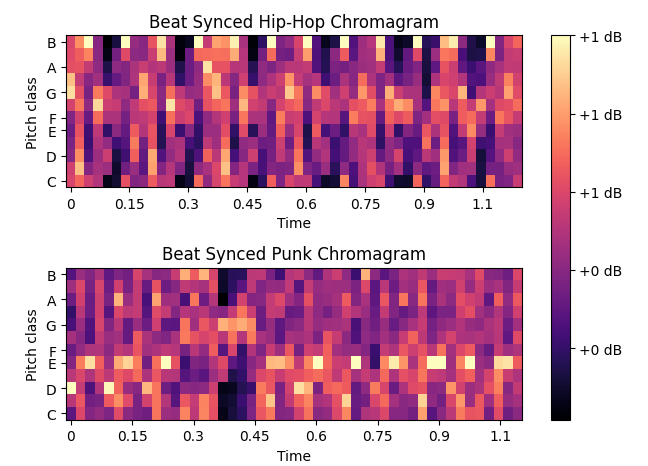
\includegraphics[width=0.7\linewidth]{images/prep_step3_chroma_beat.png}
\end{figure}

\noindent Αντίστοιχα με τα spectrograms, τα διαγράμματα είναι λιγότερο ευκρινή. Και αυτή τη φορά, η σημαντική πληροφορία διατηρείται καθώς αφενώς το μοτίβο της hip-hop παραμένει εμφανές και αφετέρου τα υπόλοιπα χαρακτηριστικά των 2 genres που σχολιάσαμε παραμένουν ευδιάκριτα. \\

\noindent Έτσι, οφείλουμε και εδώ να επισημάνουμε ότι τα πρώτα chromagrams θα παρουσιάσουν τα ίδια προβλήματα στα LSTM που θα παρουσίαζαν τα αντίστοιχα spectrograms τους (μεγάλες απαιτήσεις σε μνήμα, υπολογιστικούς πόρους, vanishing gradient, ...). Παρότι έχουμε να κάνουμε με πληροφορία για 12 νότες αντί για 140 Mel frequencies, η διάσταση των δεδομένων μας παραμένει μεγάλη. Έτσι, τα beat synced chromagrams που έχουν και εκείνα 2 τάξεις μεγέθους λιγότερα timesteps και το μεγαλύτερο ποσοστό της πληροφορίας των απλών chromograms αποτελούν μία πολύ καταλληλότερη επιλογή χαρακτηριστικών για το LSTM μας. 

\section*{Βήμα 4}
\subsection*{Ερώτημα α}
Θα ξεκινήσουμε να σχολιάζουμε τον κώδικα του tutorial κελί με κελί. \\ 

\begin{figure}[H]
	\centering
	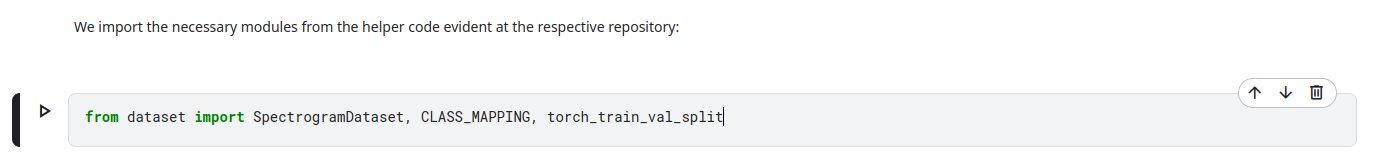
\includegraphics[width=\linewidth]{images/prep_step4_imports.png}
\end{figure}

\noindent Το πρώτο πράγμα που γίνεται είναι η εισαγωγή διάφορων κομματιών κώδικα από το repository του lab3. Συγκεκριμένα, εισάγεται ο εξής κώδικας:

\lstinputlisting[language=Python, firstline=99, lastline=159]{documents/dataset.py}

\lstinputlisting[language=Python, firstline=9, lastline=30]{documents/dataset.py}

\lstinputlisting[language=Python, firstline=33, lastline=53]{documents/dataset.py}

\noindent Θα ξεκινήσουμε σχολιάζοντας τη κλάση \textit{SpectrogramDataset}. Βασιζόμαστε στο  \href[]{https://docs.pytorch.org/tutorials/beginner/basics/data_tutorial.html#creating-a-custom-dataset-for-your-files}{documentation} της PyTorch. Ουσιαστικά, ξεκινάμε κληρωνομώντας από τη βασική κλάση Dataset της Pytorch. Η συνάρτηση \textit{\_\_init\_\_()} είναι εκείνη που εκτελείται όταν αρχικοποιείται ένα αντικείμενο τύπου \textit{SpectrogramDataset}. Στην περίπτωσή μας αυτό που γίνεται είναι ο καθορισμός για το αν πρόκειται για training ή test dataset, στη συνέχεια ενέργειες που έχουν να κάνουν με το path στο οποίο είναι αποθηκευμένα τα δεδομένα και τέλος διάφορα metadata για αυτά. \\

\noindent Θα συνεχίσουμε σχολιάζοντας την συνάρτηση \textit{\_\_getitem\_\_()}. Αυτή τη συνάρτηση χρησιμοποιούν οι DataLoaders για να δειγματοληπτήσουν το dataset και να δημιουργήσουν batches ή γενικά να εξυπηρετήσουν το data iteration στη διαδικασία εκπαίδευσης του εκάστοτε μοντέλου. \\

\noindent Συνεχίζουμε με την συνάρτηση \textit{\_\_len\_\_()}. Αυτή η συνάρτηση επιστρέφει το μέγεθος του dataset. \\

\noindent Εκτός από τις παραπάνω συναρτήσεις που ουσιαστικά επισκιάζουν εικονικές μεθόδους της κλάσης-γονέα dataset ορίζουμε και τη συνάρτηση \textit{get\_files\_labels()}. Αυτή πρακτικά με την κατάλληλη αναζήτηση στο directory που είναι αποθηκευμένο το dataset επιστρέφει τα files και τα labels που τους αντιστοιχούν σε 2 lists. \\

\noindent Το CLASS\_MAPPING δεν είναι τίποτα άλλο παρά ένα dictionary που αντιστοιχεί κλάσεις των αρχείων σε εκείνες που θα θεωρούμε ότι ανήκουν κατά την εκπαίδευση. Αυτό γίνεται διότι πολλά genres μουσικής είναι από τη φύση τους πολύ παρόμοια και έτσι δεν έχει νόημα να προσπαθήσουμε να τα διαχωρίσουμε και με το μοντέλο μας. Ένα χαρακτηριστικό παράδειγμα στο dictionary μας είναι ότι τα κλειδιά Rock και Psych-Rock οδηγούν και τα 2 στο value Rock, συγχωνεύοντας πρακτικά τις 2 αυτές κατηγορίες μουσικής. Ακόμα, οι κλάσεις που αντιστοιχούν σε value None πρακτικά εξαφανίζονται από το dataset μειώνοντας τον αριθμό των δειγμάτων. \\

\noindent Η συνάρτηση \textit{torch\_train\_val\_split()} ουσιαστικά χωρίζει το dataset σε train και test κατά ποσοστό που καθορίζεται από το χρήστη και με βάση αυτά τα 2 επιστρέφει του αντίστοιχους PyTorch DataLoaders. \\

\noindent Στη συνέχεια, αυτό που γίνεται είναι χρήση όσων εξηγήθηκαν παραπάνω για την αρχικοποίηση και την επεξήγηση κάποιων δειγμάτων από τα dataset. Αυτό, αρχικά γίνεται για χαρακτηριστικά που αντιστοιχούν στα beat synced spectrograms και στη συνέχεια για χρωμογραφήματα και τελικά για τα πλήρη - όχι beat synced δεδομένα (spectrograms και chromagrams). Στη συνέχεια εκτυπώνονται ορισμένα δείγματα τους ώστε να δούμε το μέγεθός τους, τις διαστάσεις τους και τις ετικέτες τους. Αυτά φαίνονται στις παρακάτω εικόνες:

\begin{figure}[H]
	\centering
	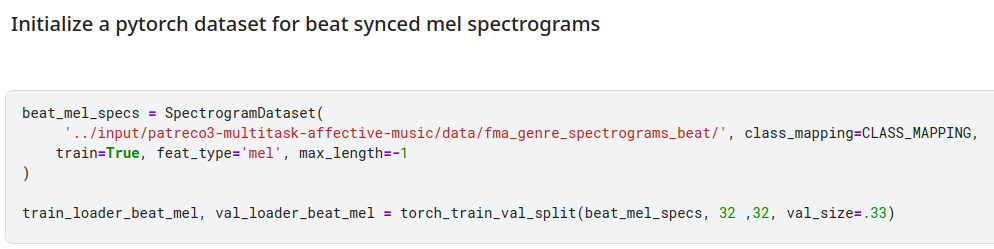
\includegraphics[width=\linewidth]{images/prep_step4_init.png}
\end{figure}

\begin{figure}[H]
	\centering
	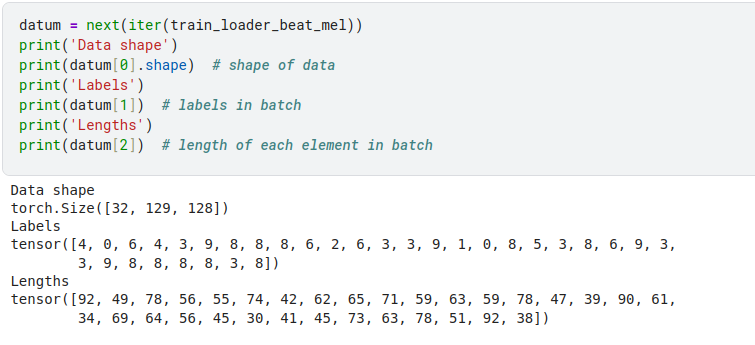
\includegraphics[width=0.8\linewidth]{images/prep_step4_print1.png}
\end{figure}

\begin{figure}[H]
	\centering
	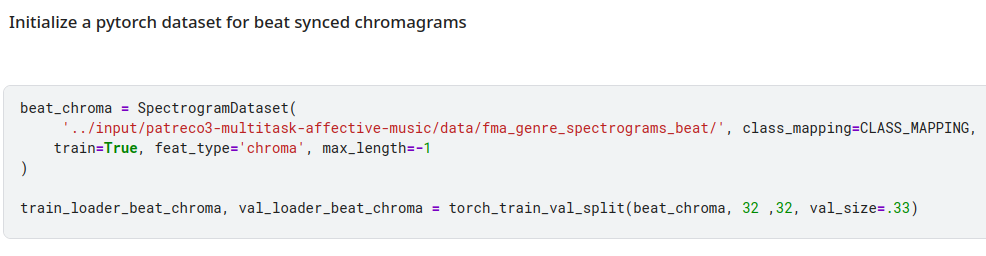
\includegraphics[width=\linewidth]{images/prep_step4_chroma.png}
\end{figure}

\begin{figure}[H]
	\centering
	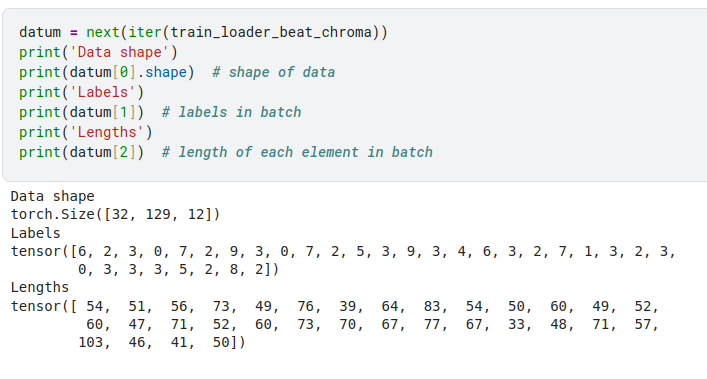
\includegraphics[width=0.8\linewidth]{images/prep_step4_print2.png}
\end{figure}

\begin{figure}[H]
	\centering
	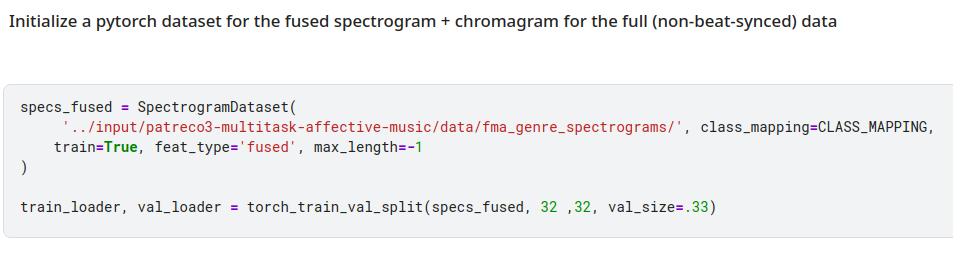
\includegraphics[width=\linewidth]{images/prep_step4_full.png}
\end{figure}

\begin{figure}[H]
	\centering
	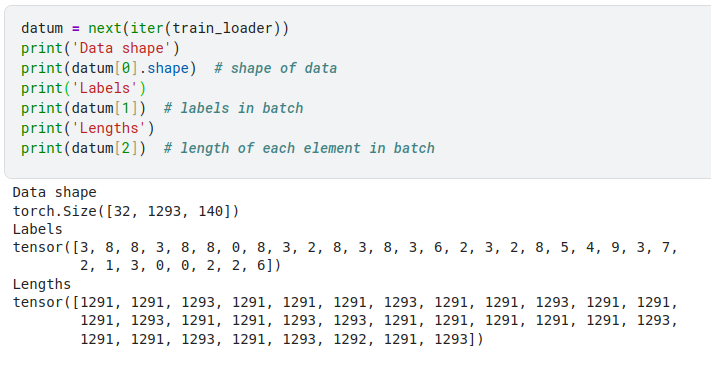
\includegraphics[width=0.8\linewidth]{images/prep_step4_print3.png}
\end{figure}

\noindent Το μόνο που μπορούμε να σχολιάσουμε και δεν είναι απευθείας προφανές από τον κώδικα και τα σχόλιά του είναι ότι τα labels από strings έχουν μετατραπεί σε ακέραιους. Μπορούμε εύκολα να δούμε ποιοι ακέραιοι αντιστοιχούν σε ποιες κλάσεις με ένα απλό inspection στο CLASS\_MAPPING που χρησιμοποιείται στην αρχικοποίση όλων των PyTorch Datasets. Για παράδειγμα: 0 -$>$ Rock, 1 -$>$ Electronic, ...  .

\subsection*{Ερωτήματα β και γ}

Για να αναπαραστήσουμε τα ιστογράμματα που ζητούνται στο ερώτημα γ, ξεκινάμε κάνοντας το εξής:

\begin{figure}[H]
	\centering
	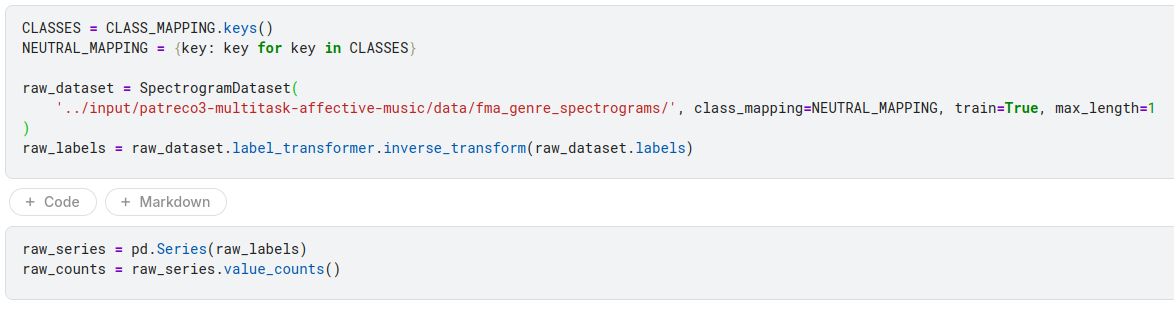
\includegraphics[width=\linewidth]{images/raw_dataset.png}
\end{figure}

\noindent Κατασκευάζουμε ένα dataset το οποίο ορίζεται με βάση το ταυτοτικό mapping στις κλάσεις. Έτσι ούτε έχουμε συγχώνευση ούτε απόρριψη κλάσεων. Από το dataset παίρνουμε τα labels εφαρμόζοντας τον αντίστροφο μετασχηματισμό που κάναμε κατά το \textit{\_\_init\_\_()}. Κατόπιν, μετράμε πόσες φορές εμφανίζεται κάθε μία (\textit{value\_counts()}). \\

\begin{figure}[H]
	\centering
	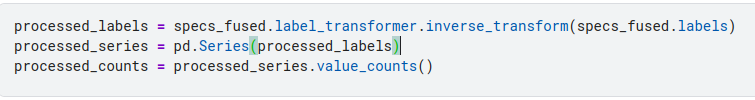
\includegraphics[width=\linewidth]{images/fused_processed_dataset.png}
\end{figure}

\noindent Το ίδιο κάνουμε και με το επεξεργασμένο dataset το οποίο έχει ήδη οριστεί στο βοηθητικό κώδικα παραπάνω (specs\_fused). \\

\noindent Προχωράμε στη σχεδίαση του histogram:

\begin{figure}[H]
	\centering
	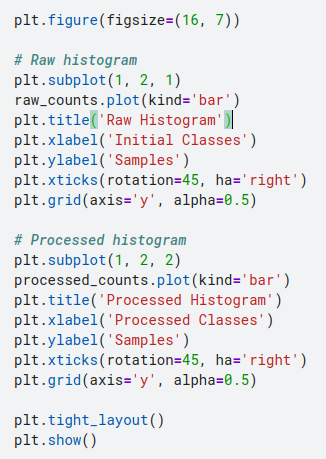
\includegraphics[width=0.3\linewidth]{images/histogram_code.png}
\end{figure}

\begin{figure}[H]
	\centering
	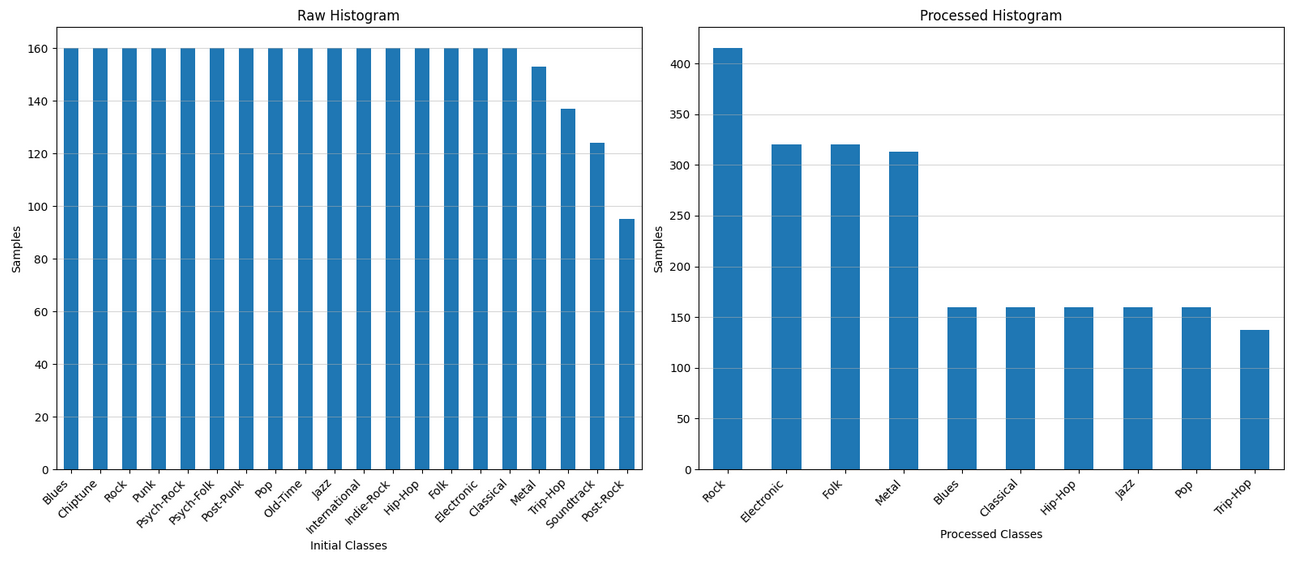
\includegraphics[width=\linewidth]{images/histograms.png}
\end{figure}

\noindent Εφαρμόζοντας ακριβώς τα ίδια βήματα και για τα άλλα 2 επεξεργασμένα dataset παίρνουμε ακριβώς τα ίδια ιστογράμματα. Για αυτό δεν υπάρχει και λόγος να τα παραθέσουμε ξανά. \\

\noindent Βλέπουμε ότι ο αριθμός των κλάσεων από 20 έχει μειωθεί σε 10. Επιπλέον, εξαιτίας των συγχωνεύσεων ο αριθμός δειγμάτων ορισμένων κλάσεων όπως της Rock έχει αυξηθεί από 160 σε πάνω από 400.

\section*{Βήμα 5}
\subsection*{Ερώτημα α}

Το LSTM που θα εκπαιδεύσουμε θα βασιστεί σε εκείνο που χρησιμοποιήσαμε στο προηγούμενο εργαστήριο. Ο κώδικας του φαίνεται παρακάτω:

\begin{figure}[H]
	\centering
	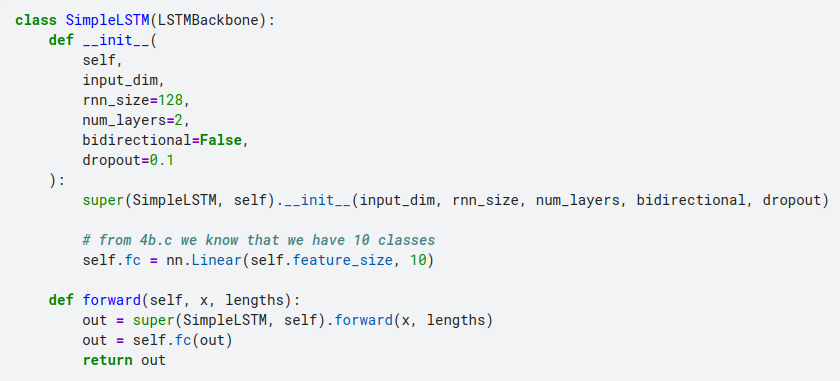
\includegraphics[width=0.9\linewidth]{images/prep_step5_lstm.png}
\end{figure}

\noindent Αξιοποιούμε τον βοηθητικό κώδικα κληρωνομώντας από την κλάση LSTMBackbone, πρακτιά ίδιο με του προηγούμενου εργαστηρίου. Το fully connected layer χρησιμοποιείται για να κάνει την τελική ταξινόμηση σε 10 κλάσεις, αριθμό που εξάγαμε εξετάζοντας τα ιστογράμματα του προηγούμενου ερωτήματος.  

\subsection*{Ερώτημα β}
Υλοποιούμε την συνάρτηση train ενσωματώνοντας την επιλογή overfit\_batch:

\lstinputlisting[language=Python]{documents/train_eval.py}

\noindent Σε περίπτωση που χρησιμοποιήσουμε το overfit\_batch το μοντέλο εκπαιδεύεται πάνω στα πρώτα 4 batches του dataloader (τυχαίο δηλαδή) μέχρι να υπερπροσαρμοστεί (loss πολύ κοντά στο 0), ενώ αν όχι ακολουθούμε την κλασσική loop εκπαίδευσης για αριθμό εποχών που ορίζεται από το χρήστη. \\

\noindent Αξίζει να σχολιάσουμε ορισμένες από τις επιλογές που έχουμε κάνει για τον αλγόριθμο εκπαίδευσής μας. Αρχικά βάζουμε το μοντέλο που εκπαιδεύουμε στη συσκευή που θα πραγματοποιήσει τους υπολογισμούς, δηλαδή τον accelerator της επιλογής μας (GPU). Χρησιμοποιούμε early stopping όπως ακριβώς και στο προηγούμενο εργαστήριο. Χρησιμοποιούμε scheduler για να ανανεώνουμε το learning rate του optimizer με βάση το loss μετά από κάθε εποχή. Έτσι, όταν έχουμε φτάσει σε κάποιο πλατό απόδοσης μειώνουμε πολύ το learning rate για να αποφύγουμε φαινόμενα αστάθειας και ταλαντώσεων. Ταυτόχρονα, στις πρώτες εποχές το learning rate είναι υψηλότερο επιτρέποντάς μας να συγκλίνουμε ταχύτερα στο ελάχιστο loss. Στη συνέχεια, διακρίνουμε 2 modes εκπαίδευσης, ένα για το αν το overfit\_batch είναι True και ένα για το αν είναι False. 

\noindent Στην περίπτωση του True, δηλαδή όταν θέλουμε να ελέγξουμε την εκπαιδευσιμότητα της αρχιτεκτονικής που επιλέξαμε για το task μας, επιλέγουμε τα 4 batches του dataloader και με ένα while loop που σταματά στο overfitting, δηλαδή accuracy 1 στα training data και loss πολύ κοντά στο 0, εκπαιδεύουμε το μοντέλο σε αυτά. Η άλλη περίπτωση κάνει κλασικό back-propagation. 

\noindent Με την συνάρτηση evaluate κάνουμε ένα απλό inference του μοντέλου και καταγράφουμε μετρικές όπως το loss και το accuracy.

\subsection*{Ερώτημα γ}
Μας ζητείται να εκπαιδεύσουμε το LSTM μας πάνω στα Mel spectrograms. Αρχικά, ξεκινάμε με την επιλογή overfit batch επιλέγοντας ένα μοντέλο με rnn\_size 256.

\begin{figure}[H]
	\centering
	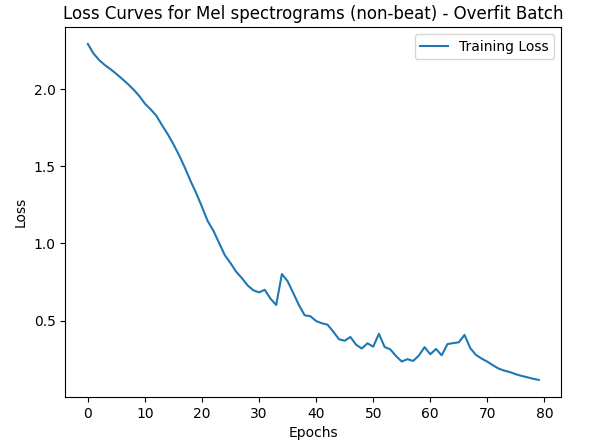
\includegraphics[width=0.6\linewidth]{images/overfit_batch_lstm_mel.png}
\end{figure}

\begin{figure}[H]
	\centering
	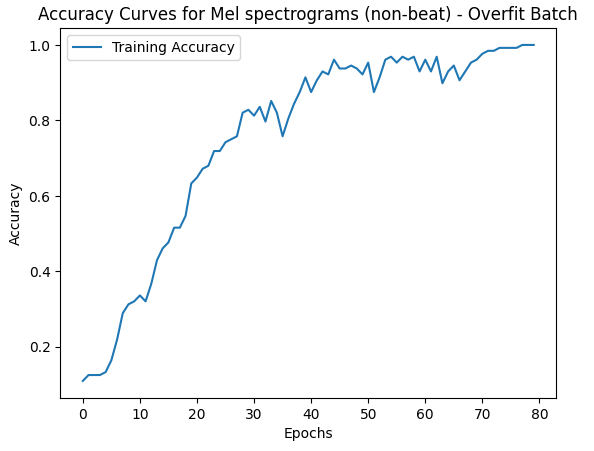
\includegraphics[width=0.6\linewidth]{images/overfit_batch_lstm_mel_acc.png}
\end{figure}

\noindent Βλέπουμε ότι πράγματι το μοντέλο υπερπροσαρμόζεται στα 4 batches γεγονός που δείχνει ότι μπορεί να αποστηθίσει τα μοτίβα τους. Επιπλέον, αξίζει να σημειώσουμε ότι αρχικά παρατηρήσαμε έντονες ταλαντώσεις και αστάθεια στην εκπαίδευση του δικτύου. Αυτό το αντιμετωπίσαμε με scheduler και με προσαρμογή της βαρύτητας κάθε κλάσης (class\_weight) δεδομένου ότι γνωρίζουμε ότι το dataset μας είναι imbalanced. Έτσι παίρνουμε μία πολύ πιο smooth εικόνα training loss από αυτή που είχαμε αρχικά.

\begin{figure}[H]
	\centering
	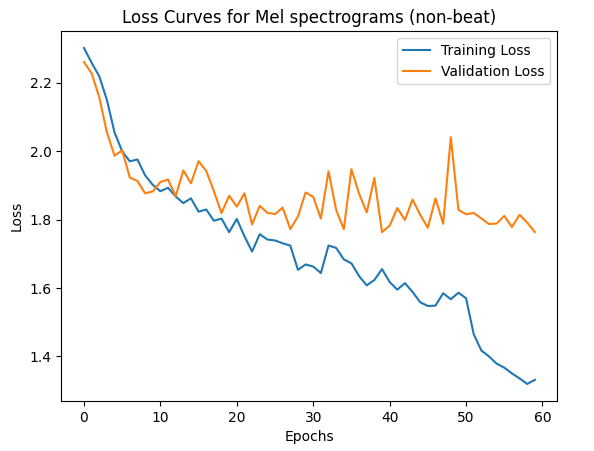
\includegraphics[width=0.6\linewidth]{images/train_mel_lstm_loss.png}
\end{figure}

\noindent Εδώ παρατηρούμε ότι το μοντέλο μας εκπαιδεύεται, αφού μειώνεται το training loss, πράγμα αναμενόμενο σύμφωνα με το προηγούμενο ερώτημα, αλλά ξεκινά να υπερπροσαρμόζεται μετά την 30η εποχή. Έτσι το early stopping που έχουμε υλοποιήσει σταματά την εκπαίδευση κάποιες εποχές αργότερα, δεδομένου ότι η απόδοσή του δεν βελτιώνεται. Αρχίζουμε να υποψιαζόμαστε το dataset είναι ενδεχομένως ανεπαρκές για την εξαγωγή χρήσιμων και γενικεύσιμων χαρακτηριστικών που θα βοηθήσουν στην ταξινόμηση.

\begin{figure}[H]
	\centering
	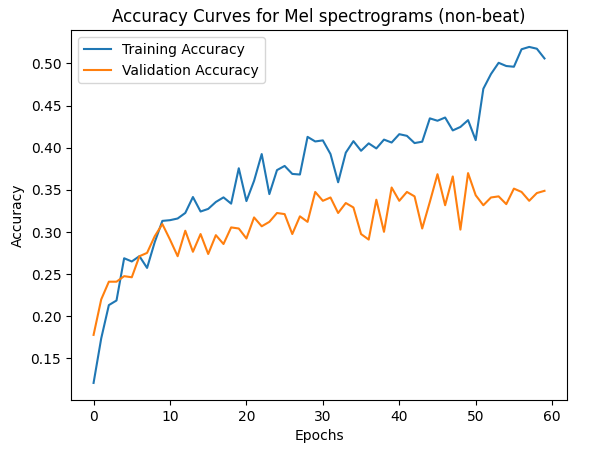
\includegraphics[width=0.6\linewidth]{images/train_mel_lstm_acc.png}
\end{figure}

\noindent Αναμενόμενα, το Accuracy ακολουθεί παρεμφερές trend με το loss. Η απόδοσή μας δεν είναι καλή (51\% στο training set και 35\% στο validation set).

\subsection*{Ερώτημα δ}
Ακολουθούμε την ίδια διαδικασία για τα τα beat-synced spectrograms. Αρχικά εκπαιδεύουμε με overfit\_batch και παίρνουμε:

\begin{figure}[H]
	\centering
	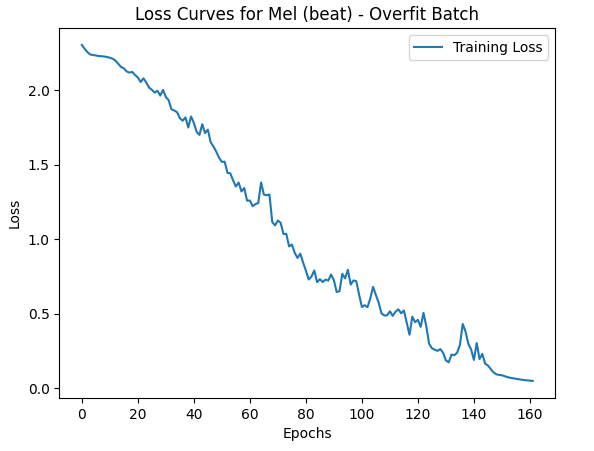
\includegraphics[width=0.5\linewidth]{images/overfit_batch_mel.png}
\end{figure}

\begin{figure}[H]
	\centering
	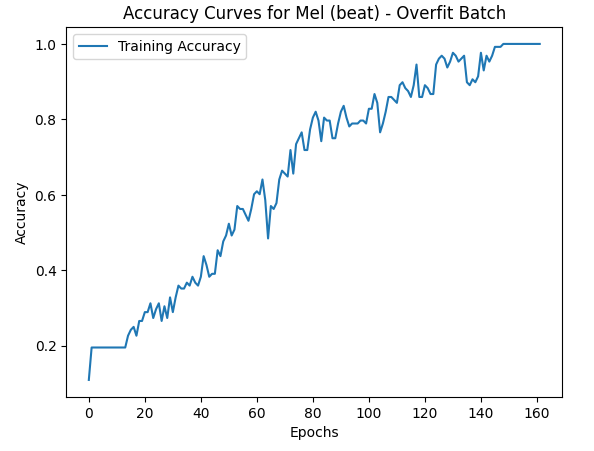
\includegraphics[width=0.5\linewidth]{images/overfit_batch_mel_acc.png}
\end{figure}

\noindent Και εδώ βλέπουμε το μοντέλο να υπερπροσαρμόζεται. Αυτό μας ενθαρρύνει να προχωρήσουμε στην εκπαίδευση του μοντέλου μας:

\begin{figure}[H]
	\centering
	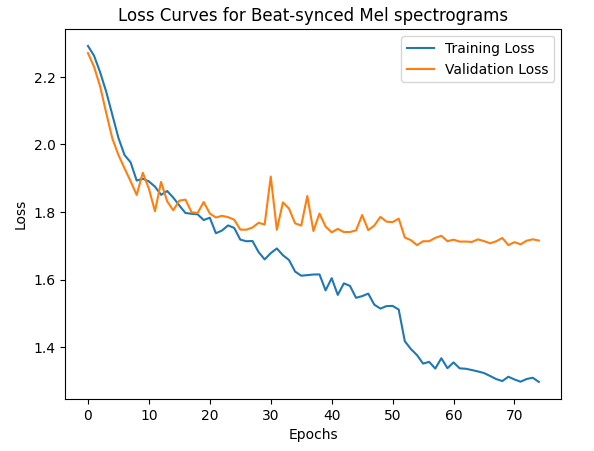
\includegraphics[width=0.6\linewidth]{images/train_beat_mel_loss.png}
\end{figure}

\begin{figure}[H]
	\centering
	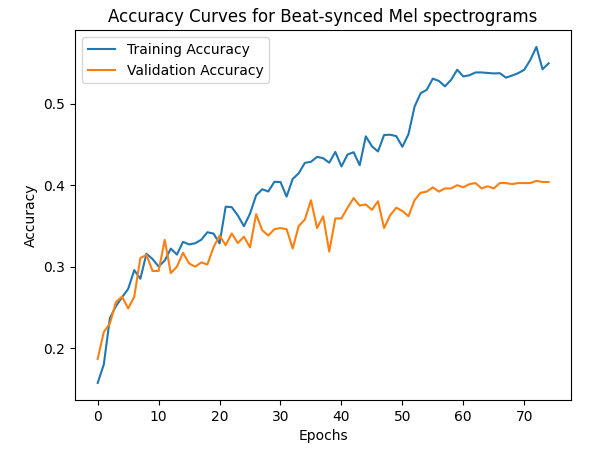
\includegraphics[width=0.6\linewidth]{images/train_beat_mel_acc.png}
\end{figure}

\noindent Για ακόμα μια φορά το μοντέλο μας εκπαιδεύεται αλλά υπερπροσαρμόζεται και σταματά να βελτιώνεται. 

\subsection*{Ερώτημα ε}

Προχωράμε στο dataset με τα χρωμογραφήματα. \\

\noindent Όπως φαίνεται στην επόμενη σελίδα το μοντέλο καταφέρνει να υπερπροσαρμοστεί στα δεδομένα, γεγονός που το καθιστά ικανό να ερμηνεύσει τα μοτίβα που εμφανίζονται στα δεδομένα εκπαίδευσης. \\

\noindent Στη συνέχεια προχωράμε στην κανονική εκπαίδευση του μοντέλου με τα αποτελέσματα να παρουσιάζονται επίσης στην επόμενη σελίδα.

\begin{figure}[H]
	\centering
	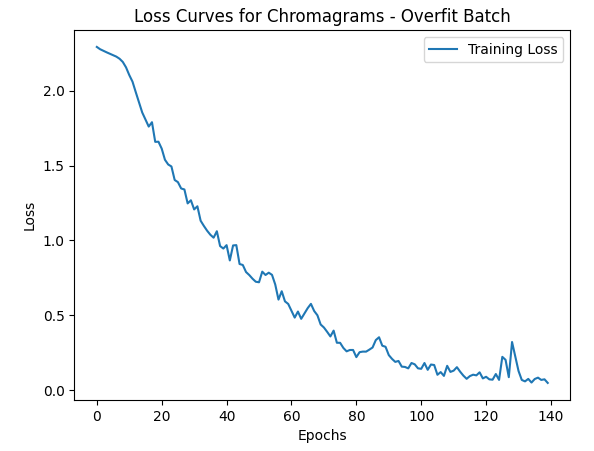
\includegraphics[width=0.6\linewidth]{images/overfit_batch_chroma.png}
\end{figure}

\begin{figure}[H]
	\centering
	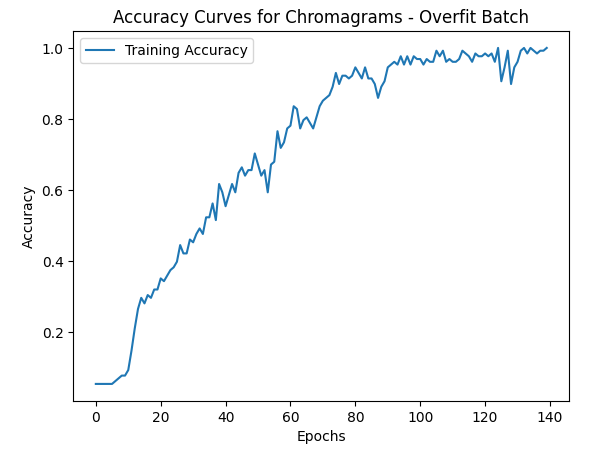
\includegraphics[width=0.6\linewidth]{images/overfit_batch_chroma_acc.png}
\end{figure}

\begin{figure}[H]
	\centering
	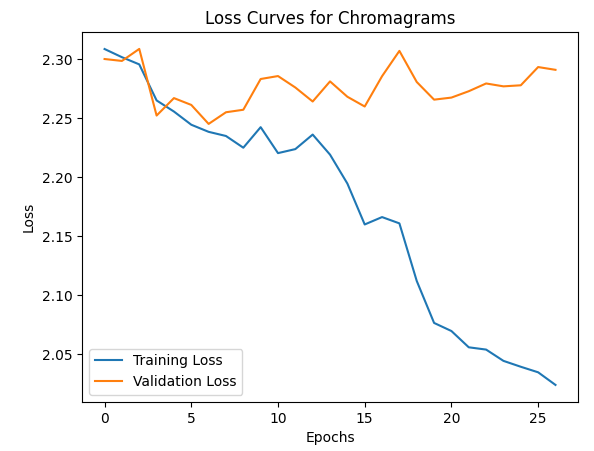
\includegraphics[width=0.6\linewidth]{images/train_chroma_loss.png}
\end{figure}

\begin{figure}[H]
	\centering
	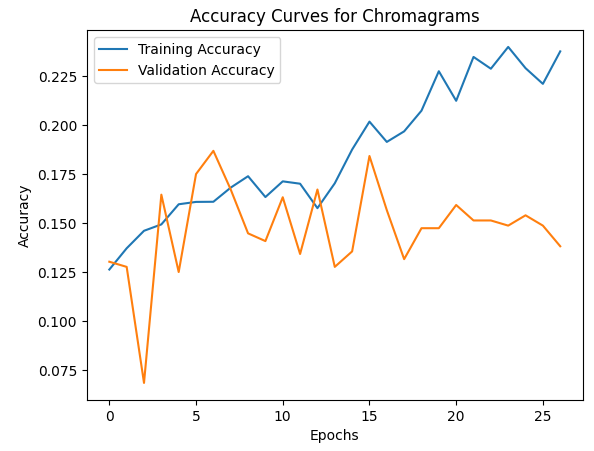
\includegraphics[width=0.6\linewidth]{images/train_chroma_acc.png}
\end{figure}

\subsection*{Ερώτημα ζ}

Τέλος, δοκιμάζουμε το μοντέλο μας με ολόκληρα τα δεδομένα μας συρραμμένα. \\

\noindent Τα αποτελέσματα της εκπαίδευσης φαίνονται παρακάτω:

\begin{figure}[H]
	\centering
	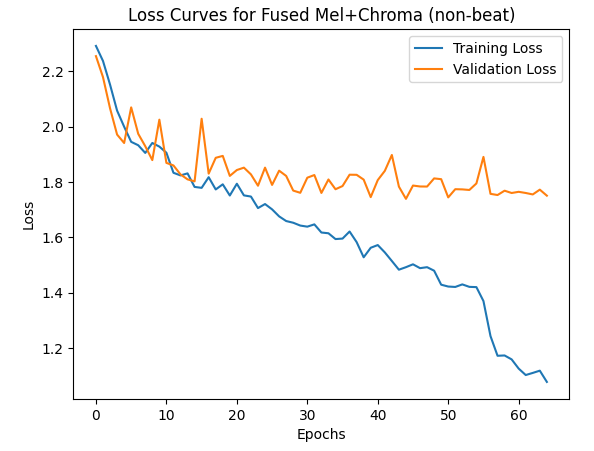
\includegraphics[width=0.55\linewidth]{images/train_fused_loss.png}
\end{figure}

\begin{figure}[H]
	\centering
	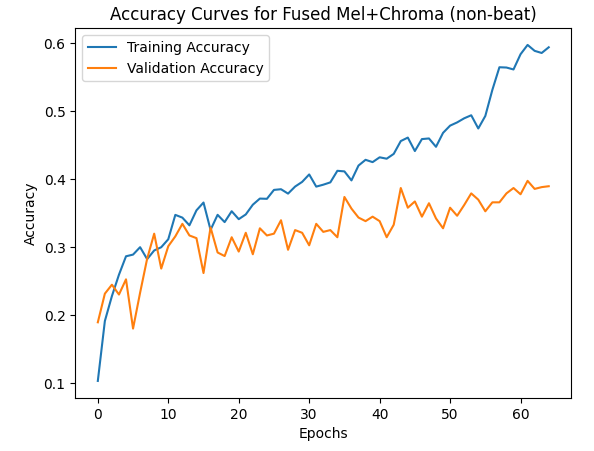
\includegraphics[width=0.55\linewidth]{images/train_fused_acc.png}
\end{figure}

\noindent Όπως βλέπουμε, πετυχαίνουμε το μεγαλύτερο validation accuracy μέχρι τώρα, αφού έχουμε τα πιο πλούσια δεδομένα, αλλά έχουμε αποτύχει να αντιμετωπίσουμε το πρόβλημα της υπερπροσαρμογής. \\

\noindent Αυτό επιβεβαιώνει την υποψία μας για αδυναμία γενίκευσης των γνώσεών μας από τα features που διαθέτουμε. Έτσι, στο κύριο μέρος του εργαστηρίου θα δοκιμάσουμε να εξάγουμε καλύτερα με ένα CNN και attention mechanism (transformer). \\

\noindent Ακολουθεί μία σύνοψη των μετρικών όλων των μοντέλων μας στο test set:

\begin{figure}[H]
	\centering
	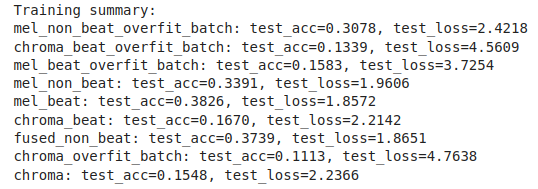
\includegraphics[width=0.8\linewidth]{images/lstm_test_summary.png}
\end{figure}

\section*{Βήμα 6}

Ο κώδικας που χρησιμοποιούμε για να υπολογίσουμε τις μετρικές που ζητούνται στα ερωτήματα του βήματος φαίνονται παρακάτω:

\lstinputlisting[language=Python]{documents/step6.py}

\noindent Ακολουθούν τα αποτελέσματα των υπολογισμών:

\lstinputlisting{documents/step6.txt}

\begin{itemize}
	\item Προκειμένου να αντιληφθούμε την σημασία των μετρικών accuracy, precision, recall και f1-score είναι χρήσιμο να αναφερθούμε στις εξής έννοιες που αφορμόνται από το πρόβλημα δυαδικής ταξινόμησης (προφανώς γενικεύονται):
	\begin{itemize}
		\item True Positive: Δείγμα που κατηγοριοποιήθηκε από το μοντέλο ως θετικό και όντως είναι σημασμένο ως θετικό (έχουμε 2 κλάσεις, οπότε ονομάζουμε αυθαίρετα τη μία θετική και την άλλη αρνητική).
		
		\item True Negative: Δείγμα που κατηγοριοποιήθηκε από το μοντέλο ως αρνητικό και όντως είναι σημασμένο ως αρνητικό.
		
		\item False Positive: Δείγμα που κατηγοριοποιήθηκε από το μοντέλο ως θετικό αλλά είναι σημασμένο ως αρνητικό.
		
		\item False Negative: Δείγμα που κατηγοριοποιήθηκε από το μοντέλο ως αρνητικό αλλά είναι σημασμένο ως θετικό.
	\end{itemize}
	
	\begin{enumerate}
		\item Η μετρική accuracy δείχνει πόσες ορθές κατηγοριοποιήσεις έγιναν από το μοντέλο μας σε όλα τα δεδομένα του.
		$$accuracy = \frac{TP+TN}{TP+TN+FP+FN}$$
		
		Το μειονέκτημά της είναι ότι μπορεί να είναι παραπλανητική για μη ισορροπημένα datasets. Για παράδειγμα, αν σε δείγμα 1000 ατόμων οι 10 είναι άρρωστοι, αλλά το μοντέλο αναγνωρίζει μόνο τον 1, φαίνεται ότι έχει accuracy $\frac{991}{1000} = 99\%$. Παρόλα αυτά το μοντέλο έχει βρει μόνο το 10\% των ασθενών έχοντας αποτύχει πλήρως στο task που πρέπει να επιλύσει.
		
		\item Για αυτό το λόγο ορίζουμε το precision. Αυτή η μετρική μας δίνει τον αριθμό θετικών δειγμάτων που εντοπίσαμε σε σχέση με το πόσα θετικά δείγματα υπάρχουν στο σύνολο του dataset, ακριβώς το παράδειγμα που συζητήσαμε πριν.
		$$precision = \frac{TP}{TP+FP}$$
		
		\item Το recall μας δίνει μια εικόνα για το ποιο ποσοστό από τα θετικά δείγματα που προβλέψαμε ήταν όντως θετικά, δηλαδή πόσα θετικά δείγματα κάναμε misclassify ως αρνητικά:
		$$recall = \frac{TP}{TP+FN}$$
		
		\item Όπως είναι φανερό από τους τύπους των μετρικών, δεν μπορούμε να μεγιστοποιήσουμε ταυτόχρονα precision και recall, υπάρχει μια σχέση tradeoff μεταξύ τους. Έτσι, πολλές φορές χρησιμοποιούμε τον αρμονικό μέσο τους, δηλαδή το f1-score:
		$$f1 = 2 \frac{Precision*Recall}{Precision+Recall}$$
	\end{enumerate}
	
	\item Micro-Averaged Metrics: Για τον υπολογισμό τους αθροίζουμε τα TP, FP, FN για όλες τις κλάσεις. Στη συνέχεια, για τα αντίστοιχα precision, recall και f1 αντί για τα απλά TP, FP, FN στους τύπους που παραθέσαμε παραπάνω χρησιμοποιούμε τα εν λόγω αθροίσματα. Αυτό που πετυχαίνουμε είναι να δώσουμε ίση βαρύτητα σε κάθε μεμονωμένο δεδομένο, κάνοντας έτσι εκείνες που έχουν τη μεγαλύτερη συχνότητα να έχουν και τη μεγαλύτερη επίδραση στο τελικό αποτέλεσμα.
	
	Macro-Averaged Metrics: Αυτή τη φορά δίνουμε ίση βαρύτητα σε κάθε κλάση ανεξάρτητα από την συχνότητα εκπροσώπησής της στο dataset. Αυτό γίνεται υπολογίζοντας το precision, recall και f1 score για την κάθε κλάση και στη συνέχεια παίρνοντας απλά τον αριθμητικό μέσο όρο τους. 
	
	Έτσι, μπορεί κανείς να αντιληφθεί ότι αν το μοντέλο μας έχει μικρότερο macro-f1 score από  micro-f1 score, δεν αποδίδει καλά σε μία ή περισσότερες μειοψηφικές κατηγορίες. Αυτό βλέπουμε να συμβαίνει καθολικά στο μοντέλο μας, αναδεικνύοντας την υποεκπροσώπηση ορισμένων πιο σπάνιων ειδών μουσικής ως κεντρικό πρόβλημα του συνόλου δεδομένων μας.
	
	\item Όπως αναδείξαμε στο πρώτο bullet, απόκλιση accuracy και f1-score μπορώ να έχω στην περίπτωση των imbalanced datasets. Πιο συγκεκριμένα, το accuracy εμφανίζεται ψηλότερο από το recall. Ερμηνεύοντας αυτή την απόκλιση, μπορούμε να συμπεράνουμε ότι το μοντέλο μας δεν είναι αποτελεσματικό στη πρόβλεψη της σπάνιας κατηγορίας.
	
	\item Είναι η multi-class εκδοχή του προηγούμενου bullet. Είναι ενδεικτικό ανισορροπίας στο σύνολο δεδομένων και κακής απόδοσης στις κλάσεις που εμφανίζονται σπανιότερα. 
	
	\item Υπάρχουν ορισμένα προβλήματα στα οποία το precision μπορεί να μας ενδιαφέρει περισσότερο από το recall και αντίστροφα. Εξαρτάται από τη βαρύτητα που προσίδουμε σε κάθε τύπο σφάλματος στο task που καλούμαστε να επιλύσουμε. Ειδικότερα, το precision μας ενδιαφέρει αν αξιολογούμε το κόστος ενός FP ως υψηλό. Ένα τέτοιο παράδειγμα είναι το spam detection, καθώς δε θα θέλαμε να κατηγοριοποιήσουμε ένα κρίσιμο email ως spam. 
	
	Αντίστοιχα, όταν δίνουμε μεγαλύτερη σημασία στο recall υποδηλώνουμε ότι το κόστος του FN είναι υψηλό. Τέτοιο χαρακτηριστικό παράδειγμα είναι οι ιατρικές διαγνώσεις. Είναι προτιμότερο να κατηγοριοποιήσω μη ασθενείς ως ασθενείς παρά το αντίστροφο.
	
	Σε αυτές τις περιπτώσεις καλές τιμές accuracy και f1 score δεν είναι αρκετές. Αυτό συμβαίνει διότι το accuracy δίνει ίδια βαρύτητα σε όλες τις κλάσεις, πράγμα που δεν το θέλουμε πάντα, ενώ, το f1-score δίνει την ίδια βαρύτητα στο precision και το recall, κάτι που συχνά δεν είναι επίσης επιθυμητό όπως εξηγήσαμε προηγουμένως.  
\end{itemize}
